\chapter{Phân tích hệ thống}

Haitay là một hệ thống hai lớp: thiết bị nằm trên bàn luyện tập và phần mềm chạy trên máy tính. Mỗi lượt solve bắt đầu bằng một cú chạm tay của người chơi và kết thúc bằng một điểm dữ liệu trên biểu đồ tiến bộ.

\section{Mô tả chung}
Haitay phục vụ một người chơi ngồi luyện tập tại bàn, với một thiết bị và một máy tính trong tầm tay. Toàn bộ dữ liệu nằm trên hai thiết bị đó, và người chơi thấy tiến bộ của mình mà không cần ghi chép hay tính toán.

\subsection{Tình huống sử dụng}
Một buổi luyện tập của người chơi diễn ra theo trình tự quen thuộc. Người chơi bật thiết bị và giải liên tiếp nhiều lượt trong một session. Sau mỗi lượt, thiết bị hiện ngay thời gian cùng các chỉ số best, mean, Ao5, Ao12 và Ao100, nên người chơi nắm được phong độ ngay tại bàn. Khi kết thúc buổi, hoặc khi người khác muốn dùng chung thiết bị, dữ liệu được đồng bộ sang máy tính, nơi nó được gắn với một người dùng và lưu lâu dài. Lúc ngồi trước máy tính, người chơi mở dashboard để xem xu hướng qua nhiều tuần và nhiều tháng.

\subsection{Hai lớp của hệ thống}
Hệ thống chia việc cho hai lớp, và mỗi lớp giữ một loại dữ liệu có vòng đời riêng. Thiết bị giữ các session gần nhất mà không biết chủ của chúng, đủ để tính Ao100 và không phải sao lưu liên tục. Máy tính gắn session với người dùng và giữ dữ liệu của mọi người dùng trong nhiều tháng và nhiều năm.

\begin{table}[H]
    \centering
    \renewcommand{\arraystretch}{1.5}
    \caption{Vai trò của hai lớp trong Haitay}
    \label{tab:layers}
    \begin{tabular}{>{\bfseries\raggedright\arraybackslash}m{2.8cm} >{\raggedright\arraybackslash}m{5.8cm} >{\raggedright\arraybackslash}m{5.6cm}}
        \toprule
        \rowcolor{haitayblue}
        \textcolor{white}{Lớp} & \textcolor{white}{Nhiệm vụ} & \textcolor{white}{Dữ liệu giữ} \\
        \midrule
        \rowcolor{haitayblue!8}
        Thiết bị & Đo thời gian solve, hiển thị thống kê, lưu trung hạn, gửi dữ liệu khi đồng bộ & Hơn 100 lượt solve gần nhất, tổ chức theo session, không kèm thông tin người dùng \\
        Máy tính & Nhận và xác nhận dữ liệu, gắn session với người dùng, lưu lâu dài, vẽ dashboard & Toàn bộ lịch sử và danh tính của mọi người dùng \\
        \bottomrule
    \end{tabular}
\end{table}

\subsection{Phạm vi}
Haitay gồm một thiết bị và một máy tính, kết nối trực tiếp với nhau. Dữ liệu ở lại trên chính hai thiết bị đó, nên hệ thống hoạt động đầy đủ mà không cần dịch vụ trung gian nào. Danh tính chỉ tồn tại trên máy tính, và xác thực người dùng là tùy chọn, dành cho trường hợp nhiều người chia sẻ một máy tính. Haitay là công cụ luyện tập hằng ngày và giữ vai trò bổ trợ cho các timer dùng trong thi đấu.

% Bài tập 6 chỉ gồm mục 2.1 và 2.4: bai6.tex định nghĩa \skipcontext và \skipdevice.
\ifdefined\skipcontext\else\section{Bối cảnh}
\label{sec:context}
Haitay không xuất hiện từ con số không, vì nó kế thừa một công cụ mà mọi cuber đều quen tay. Hiểu cách công cụ ấy hoạt động giúp thấy rõ Haitay giữ lại điều gì và thay đổi điều gì.

\subsection{Stackmat}
Stackmat là bộ hẹn giờ chuẩn tại các giải speedcubing, với dáng thanh ngang dễ nhận ra. Hình~\ref{fig:stackmat} cho thấy cấu tạo của nó: hai pad màu đen nằm ở hai đầu thân máy, mỗi pad in một biểu tượng bàn tay để chỉ chỗ đặt lòng bàn tay, còn mặt hiển thị và các nút điều khiển nằm gọn ở phần giữa.

\begin{figure}[htbp]
    \centering
    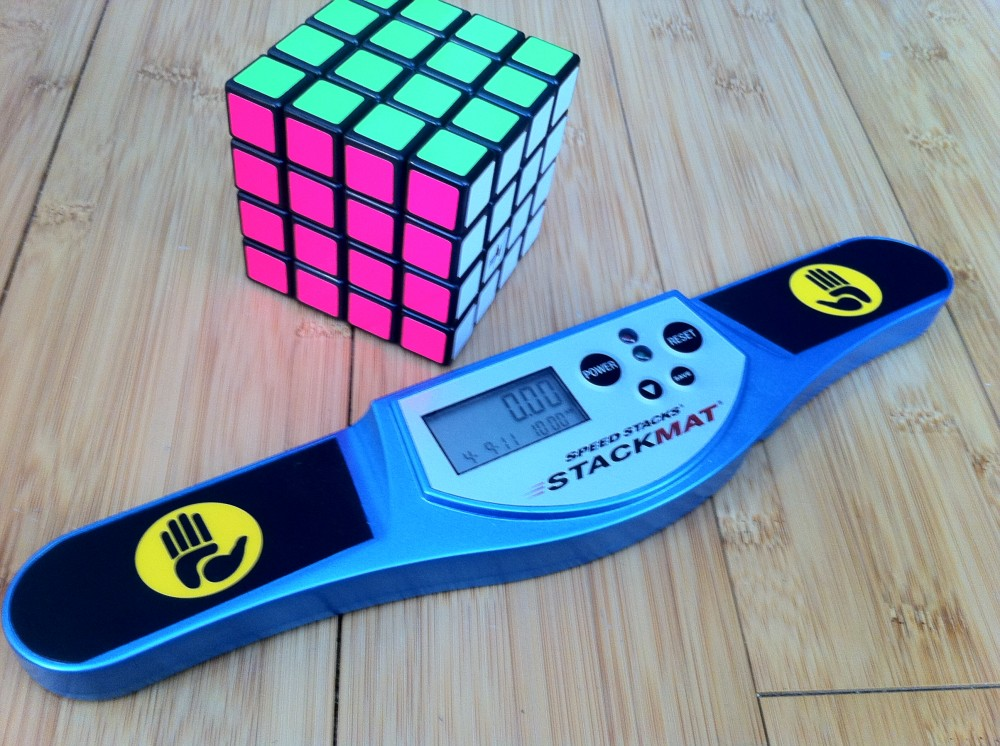
\includegraphics[width=0.78\textwidth]{figures/stackmat.jpg}
    \caption{Stackmat đặt cạnh một khối Rubik 4$\times$4. Hai pad ở hai đầu mang biểu tượng bàn tay. Ảnh của Protocoldoug, giấy phép CC0, nguồn Wikimedia Commons.}
    \label{fig:stackmat}
\end{figure}

Nguyên tắc vận hành của Stackmat xoay quanh việc cố định cả hai tay. Trước lượt solve, người chơi đặt đồng thời hai bàn tay lên hai pad. Khi thiết bị nhận ra cả hai tay đã chạm, nó chuyển sang trạng thái sẵn sàng. Người chơi nhấc một hoặc cả hai tay để bắt đầu giải, và đồng hồ chạy ngay tại thời điểm nhả pad. Giải xong khối, họ đặt cả hai tay trở lại pad để dừng đồng hồ.\footnote{Theo quy tắc StackMat Pro của WSSA: \url{https://www.thewssa.com/docs/rules_rules.pdf}.}

Cách cố định này giải quyết hai vấn đề cùng lúc. Trước hết, cả hai tay đều rời khối Rubik trước khi đồng hồ chạy, nên mọi người bắt đầu từ cùng một điểm xuất phát. Kế đó, người chơi phải buông khối bằng cả hai tay mới dừng được đồng hồ, nên thời gian dừng phản ánh đúng lúc khối được giải xong. Một nút bấm duy nhất khó đạt được hai điều này, và đó là lý do cơ chế hai pad được giữ lại ở Haitay.

% Chừa chỗ: luật thi đấu WCA liên quan đến bấm giờ, bổ sung sau.
\fi
\ifdefined\skipdevice\else\section{Lớp thiết bị}
Thiết bị là nơi mỗi lượt solve được ghi lại, nên độ tin cậy của cả hệ thống bắt đầu từ đây. Một thiết bị bấm giờ tốt là thiết bị mà người chơi có thể quên đi, để toàn bộ sự chú ý dành cho khối Rubik trên tay.

\subsection{Đặc tả thiết bị}
Haitay giữ nguyên nguyên tắc cố định hai tay của Stackmat (mục~\ref{sec:context}) và thu gọn phần cứng quanh nó. Các chi tiết hình dạng dưới đây là thiết kế dự kiến của nhóm. Thân máy là một thanh nhựa in 3D, dài vừa đủ để hai bàn tay đặt thoải mái ở hai đầu. Mỗi pad là một miếng lá đồng dán trên mặt vỏ, và vi điều khiển nhận biết tay chạm hay nhả qua cảm biến chạm điện dung. Màn hình nằm ở giữa thân máy, hiển thị thời gian và các chỉ số thống kê. Các nút chức năng được đặt lõm và tránh khoảng giữa hai pad, vì ngón cái dễ bấm nhầm vào đó khi tay đang đặt trên pad. Thiết bị lấy điện qua cổng USB-C 5~V từ bộ sạc hoặc sạc dự phòng và không có pin nuôi thiết bị, nên thân máy gọn và không cần mạch sạc. Một pin cúc áo nhỏ chỉ giữ đồng hồ thực (mục~\ref{sec:rtc}).

Mỗi lượt solve đưa thiết bị đi qua bốn trạng thái, như Bảng~\ref{tab:states} mô tả. Sau khi người chơi xác nhận kết quả là OK, +2 hay DNF, thiết bị lưu bản ghi và quay về trạng thái chờ cho lượt kế tiếp.

\begin{table}[H]
    \centering
    \renewcommand{\arraystretch}{1.5}
    \caption{Bốn trạng thái của thiết bị trong một lượt solve}
    \label{tab:states}
    \begin{tabular}{>{\bfseries\raggedright\arraybackslash}m{2.4cm} >{\raggedright\arraybackslash}m{5.6cm} >{\raggedright\arraybackslash}m{6.2cm}}
        \toprule
        \rowcolor{haitayblue}
        \textcolor{white}{Trạng thái} & \textcolor{white}{Điều kiện chuyển vào} & \textcolor{white}{Màn hình hiển thị} \\
        \midrule
        \rowcolor{haitayblue!8}
        Chờ & Vừa bật máy, hoặc vừa ghi xong lượt solve trước & Thời gian lượt trước cùng Ao5 và Ao12 \\
        Sẵn sàng & Cả hai pad được chạm liên tục 1,5 giây & Tín hiệu cho phép bắt đầu \\
        \rowcolor{haitayblue!8}
        Chạy & Người chơi nhấc ít nhất một tay khỏi pad & Thời gian đang chạy, hiển thị gọn để không phân tán người chơi \\
        Dừng & Cả hai pad được chạm lại & Thời gian chính thức với độ phân giải dưới 1~ms, chờ chọn OK, +2 hoặc DNF \\
        \bottomrule
    \end{tabular}
\end{table}

\subsection{Đại lượng đo}
Từ cơ chế trên, đại lượng thiết bị cần đo là thời gian solve, tức khoảng thời gian từ lúc người chơi nhả pad đến lúc cả hai pad được chạm lại. Trạng thái chạm của từng pad là tín hiệu phụ, dùng để điều khiển các trạng thái ở Bảng~\ref{tab:states}. Các chỉ số best, mean, Ao5, Ao12 và Ao100 không phải kết quả đo trực tiếp, vì thiết bị tính chúng từ những thời gian đã lưu.

Về độ chính xác, cần phân biệt hai con số. Firmware ghi mốc thời gian với độ phân giải dưới 1~ms nhờ bộ định thời phần cứng 1~MHz, và đây là mục tiêu lý thuyết của thiết bị. Cảm biến chạm cần thêm 2 đến 10~ms để phát hiện tay chạm hoặc nhả. Nhóm chấp nhận khoảng này vì đo độ trễ tuyệt đối đòi hỏi một thiết bị tham chiếu rất phức tạp. Thêm vào đó, sai lệch của thời gian solve chỉ là chênh lệch giữa độ trễ ở cạnh nhả và độ trễ ở cạnh chạm, nên nhỏ hơn độ trễ lớn nhất trong hai cạnh.

\begin{table}[H]
    \centering
    \renewcommand{\arraystretch}{1.5}
    \caption{Các đại lượng thiết bị đo}
    \label{tab:measured}
    \begin{tabular}{>{\bfseries\raggedright\arraybackslash}m{3.4cm} >{\raggedright\arraybackslash}m{5.6cm} >{\raggedright\arraybackslash}m{5.2cm}}
        \toprule
        \rowcolor{haitayblue}
        \textcolor{white}{Đại lượng} & \textcolor{white}{Nguồn đo} & \textcolor{white}{Công dụng} \\
        \midrule
        \rowcolor{haitayblue!8}
        Thời gian solve & Hiệu hai mốc thời gian từ bộ định thời phần cứng 1~MHz & Dữ liệu chính, gửi lên máy tính \\
        Trạng thái hai pad & Cảm biến chạm, hai kênh & Điều khiển các trạng thái chờ, sẵn sàng, chạy, dừng \\
        \bottomrule
    \end{tabular}
\end{table}

\subsection{Cảm biến}
Cảm biến của Haitay chỉ cần trả lời một câu hỏi: pad đang có tay chạm hay không. Nhóm chọn cảm biến chạm điện dung có sẵn trong ESP32-S3. Khi tay chạm vào miếng lá đồng, điện dung của miếng đồng tăng lên đủ để vi điều khiển phát hiện. Driver của ESP-IDF gọi hàm xử lý đúng lúc pad được kích hoạt và lúc pad được nhả, và firmware ghi mốc thời gian ngay trong hàm đó. Nếu cảm biến có sẵn thiếu ổn định, nhóm dùng MPR121, một chip cảm biến chạm ngoài giao tiếp qua I2C, để thay thế.

Ngón tay hiếm khi chạm hay nhả một cách dứt khoát, nên tín hiệu cần được xử lý kỹ. Driver của ESP-IDF cung cấp sẵn ba công cụ cho việc này: ngưỡng kích hoạt đi kèm ngưỡng hysteresis để xác định lúc pad được nhả, bộ đếm chống nảy và bộ lọc nhiễu. Nhờ ngưỡng hysteresis, tín hiệu dao động quanh một mức không làm pad bật tắt liên tục. Thiết bị chỉ vào trạng thái sẵn sàng khi cả hai pad cùng chạm liên tục 1,5 giây, đủ lâu để bỏ qua những lần chạm vô tình, và chỉ dừng đồng hồ khi cả hai pad cùng được chạm lại. Cách xử lý này giữ cho mốc bắt đầu và mốc dừng khớp với ý định thật của người chơi.

\subsection{Tiêu chí lựa chọn}
Nhóm cân nhắc bốn phương án cảm biến theo năm tiêu chí của môn học. Các con số về độ trễ lấy từ báo cáo nghiên cứu nền và mới ở mức ước lượng, nên nhóm sẽ đo lại trên thiết bị thật.

\begin{table}[H]
    \centering
    \small
    \renewcommand{\arraystretch}{1.4}
    \caption{So sánh phương án cảm biến theo năm tiêu chí}
    \label{tab:sensor-criteria}
    \begin{tabular}{>{\bfseries\raggedright\arraybackslash}m{2.0cm} >{\raggedright\arraybackslash}m{3.1cm} >{\raggedright\arraybackslash}m{2.9cm} >{\raggedright\arraybackslash}m{2.7cm} >{\raggedright\arraybackslash}m{2.7cm}}
        \toprule
        \rowcolor{haitayblue}
        \textcolor{white}{Tiêu chí} & \textcolor{white}{Chạm có sẵn trong ESP32-S3 (chọn)} & \textcolor{white}{MPR121 (dự phòng)} & \textcolor{white}{TTP223 (loại)} & \textcolor{white}{Công tắc cơ (loại)} \\
        \midrule
        \rowcolor{haitayblue!8}
        Độ chính xác & Hàm xử lý lúc chạm và nhả chạy thẳng trong firmware; độ trễ cảm biến 2 đến 10~ms mỗi cạnh (ước lượng), đo và hiệu chỉnh được & Có chân ngắt riêng nhưng thêm một lớp giao tiếp I2C; độ trễ cần đo & Thời gian đáp ứng 60 đến 220~ms, vượt xa độ phân giải 1~ms & Phản hồi nhanh, tiếp điểm nảy nên cần lọc bằng phần mềm \\
        Độ bền & Không có bộ phận chuyển động; cần hiệu chỉnh lại ngưỡng khi độ ẩm đổi & Giống phương án chọn, có tự theo dõi mức nền & Không có bộ phận chuyển động & Tiếp điểm mòn theo số lần bấm \\
        \rowcolor{haitayblue!8}
        Điện năng & Nằm trong chip, không thêm linh kiện & Thêm một chip ngoài, dòng nhỏ & Thấp & Gần như bằng 0 \\
        Chi phí & Chỉ tốn lá đồng & Khoảng 25.000 đồng mỗi chip & Thấp & Thấp \\
        \rowcolor{haitayblue!8}
        Môi trường & Trong nhà, tay có mồ hôi; vỏ nhựa in 3D cách điện; nhiễu từ bộ sạc USB có thể làm lệch ngưỡng & Giống phương án chọn & Giống phương án chọn & Không phụ thuộc độ ẩm, nhưng cảm giác tay khác Stackmat \\
        \bottomrule
    \end{tabular}
\end{table}

Nếu thử nghiệm đầu tiên cho thấy cảm biến có sẵn kích hoạt sai, nhóm chuyển sang MPR121. Ngưỡng chạm lệch theo độ ẩm, nên firmware hiệu chuẩn lại ngưỡng mỗi lần khởi động. Với cách xử lý đó, cảm biến chạm có sẵn giữ được ba ưu thế: tín hiệu đi qua ít khâu nhất, không tốn thêm linh kiện và cho phép ghi mốc thời gian ngay trong hàm xử lý.

\subsection{Vi điều khiển}
Vi điều khiển quyết định thiết bị chạy ổn định được bao lâu, nên nhóm xếp độ bền và độ ổn định lâu dài lên trên giá thành. Bảng~\ref{tab:mcu} đặt ba ứng viên cạnh nhau: ESP32-S3, STM32WB55 và Raspberry Pi Pico 2 W.

\begin{table}[H]
    \centering
    \small
    \renewcommand{\arraystretch}{1.4}
    \caption{So sánh ba vi điều khiển có Bluetooth LE}
    \label{tab:mcu}
    \begin{tabular}{>{\bfseries\raggedright\arraybackslash}m{2.6cm} >{\raggedright\arraybackslash}m{3.7cm} >{\raggedright\arraybackslash}m{3.7cm} >{\raggedright\arraybackslash}m{3.4cm}}
        \toprule
        \rowcolor{haitayblue}
        \textcolor{white}{Tiêu chí} & \textcolor{white}{ESP32-S3 (chọn)} & \textcolor{white}{STM32WB55 (dự phòng)} & \textcolor{white}{Pico 2 W (loại)} \\
        \midrule
        \rowcolor{haitayblue!8}
        Cung ứng dài hạn & Cam kết ít nhất 12 năm kể từ 1/1/2021 & Trong danh sách cam kết 10 năm của ST, đến tháng 1 năm 2036 & Sản xuất đến ít nhất tháng 1 năm 2040 \\
        Cảm biến chạm & Có sẵn, 14 kênh & Có sẵn, tối đa 18 kênh (trừ gói 48 chân UFQFPN) & Không nêu trong thông số, cần thêm MPR121 \\
        \rowcolor{haitayblue!8}
        Bluetooth LE & Bản 5.0 & Bản 5.4 & Bản 5.2 \\
        Nhiệt độ làm việc & $-40$ đến 85~$^{\circ}$C (module N8) & $-40$ đến 105~$^{\circ}$C & $-20$ đến 85~$^{\circ}$C \\
        \rowcolor{haitayblue!8}
        Pin dự phòng cho đồng hồ thực & Không có chân riêng, cần chip đồng hồ ngoài & Có chân VBAT, nhận pin cúc áo hoặc siêu tụ & Không nêu trong thông số \\
        Bộ nhớ chương trình & 8~MB flash, 512~KB SRAM & Tối đa 1~MB flash, 256~KB SRAM & 4~MB flash, 520~KB SRAM \\
        \bottomrule
    \end{tabular}
\end{table}

Nhóm chọn module ESP32-S3-WROOM-1 bản N8. Pico 2 W bị loại trước vì cần thêm một chip cảm biến chạm ngoài. Giữa hai ứng viên còn lại, STM32WB55 dẫn trước về cam kết cung ứng, dải nhiệt độ, phiên bản Bluetooth LE và có chân VBAT cho đồng hồ thực. ESP32-S3 được chọn vì hệ sinh thái trưởng thành hơn và đã có các dự án bấm giờ mã nguồn mở dùng chính cặp cảm biến chạm với Bluetooth LE, nên rủi ro tích hợp thấp hơn. Bản N8 làm việc trong dải $-40$ đến 85~$^{\circ}$C, rộng hơn các bản có thêm PSRAM chỉ chịu tới 65~$^{\circ}$C, và cam kết cung ứng 12 năm dài hơn nhiều so với vòng đời của một thiết bị luyện tập. STM32WB55 là phương án thay thế khi nhóm ưu tiên độ bền dài hạn hơn sự thuận tiện khi phát triển.

\subsection{Bộ nhớ lưu trữ}
Thiết bị không có pin, nên người chơi rút cáp là mất điện ngay, và lượt solve vừa ghi phải sống sót qua khoảnh khắc đó. Nhóm vì vậy chọn bộ nhớ theo khả năng chịu mất điện đột ngột trước, rồi mới đến dung lượng và giá. Yêu cầu dung lượng khá khiêm tốn: hơn 100 lượt solve, mỗi lượt 16 byte, tức chưa đến 2~KB. Bảng~\ref{tab:storage} so sánh ba phương án.

\begin{table}[H]
    \centering
    \small
    \renewcommand{\arraystretch}{1.4}
    \caption{So sánh ba phương án lưu nhật ký solve}
    \label{tab:storage}
    \begin{tabular}{>{\bfseries\raggedright\arraybackslash}m{2.6cm} >{\raggedright\arraybackslash}m{3.7cm} >{\raggedright\arraybackslash}m{3.9cm} >{\raggedright\arraybackslash}m{3.2cm}}
        \toprule
        \rowcolor{haitayblue}
        \textcolor{white}{Tiêu chí} & \textcolor{white}{FRAM FM24CL64B (chọn)} & \textcolor{white}{Flash W25Q128JV và LittleFS (dự phòng)} & \textcolor{white}{EEPROM 24LC256 (loại)} \\
        \midrule
        \rowcolor{haitayblue!8}
        Độ bền ghi & $10^{14}$ lần ghi & 100.000 chu kỳ xóa ghi mỗi sector, LittleFS dàn đều hao mòn & 1.000.000 chu kỳ mỗi page \\
        Lưu giữ dữ liệu & Tối thiểu 10 năm ở 85~$^{\circ}$C, 151 năm ở 65~$^{\circ}$C & Hơn 20 năm & Hơn 200 năm \\
        \rowcolor{haitayblue!8}
        Tốc độ ghi & Ghi ngay trong lúc truyền, không phải chờ & Ghi page 0,4 đến 3~ms; xóa sector 45 đến 400~ms & Chờ tối đa 5~ms mỗi lần ghi \\
        Mất điện đột ngột & Gần như không có khoảng chờ để dở dang & LittleFS được thiết kế để chịu mất điện ngẫu nhiên & Mất điện trong 5~ms chờ có thể hỏng page, CRC phát hiện được \\
        \rowcolor{haitayblue!8}
        Dung lượng & 8~KB, chứa 512 bản ghi & 16~MB & 32~KB \\
        Chi phí & Cao nhất (ước lượng) & Thấp & Thấp \\
        \bottomrule
    \end{tabular}
\end{table}

Nhóm chọn FRAM cho nhật ký solve. Dữ liệu vào bộ nhớ ngay trong lúc truyền nên khoảnh khắc rút cáp hầu như không để lại bản ghi dở dang, và mã \texttt{CRC16} trong mỗi bản ghi phát hiện phần còn lại. Thời gian lưu giữ của FRAM ngắn hơn EEPROM, nhưng vẫn vượt xa nhu cầu vì dữ liệu được đồng bộ sang máy tính sau mỗi buổi luyện tập. Dung lượng 8~KB chứa 512 bản ghi, gấp hơn năm lần mức tối thiểu. Flash trong module ESP32-S3 vẫn lưu firmware và cấu hình, đồng thời là nhật ký dự phòng nếu FRAM khó tìm nguồn cung. EEPROM bị loại vì mỗi lần ghi phải chờ tới 5~ms, đúng khoảng thời gian mà một lần rút cáp có thể làm hỏng page đang ghi.

\subsection{Đồng hồ thực}
\label{sec:rtc}
Dashboard vẽ tiến bộ theo ngày và theo tháng, nên mỗi lượt solve cần một mốc giờ thực đáng tin. Thiết bị không có pin nuôi, vì vậy giờ sẽ biến mất ngay khi người chơi rút cáp nếu không có nguồn riêng giữ đồng hồ. Bảng~\ref{tab:rtc} so sánh các cách giải quyết.

\begin{table}[H]
    \centering
    \renewcommand{\arraystretch}{1.5}
    \caption{So sánh bốn cách giữ giờ thực}
    \label{tab:rtc}
    \begin{tabular}{>{\bfseries\raggedright\arraybackslash}m{4.0cm} >{\raggedright\arraybackslash}m{3.4cm} >{\raggedright\arraybackslash}m{6.8cm}}
        \toprule
        \rowcolor{haitayblue}
        \textcolor{white}{Phương án} & \textcolor{white}{Giữ giờ khi rút cáp} & \textcolor{white}{Nhận xét} \\
        \midrule
        \rowcolor{haitayblue!8}
        DS3231 và pin cúc áo CR2032 (chọn) & Có, qua ngõ pin dự phòng & Sai số $\pm 2$~ppm ở 0 đến 40~$^{\circ}$C, tức khoảng 0,17 giây mỗi ngày; giao tiếp I2C chung bus với FRAM \\
        Chỉ đặt giờ bằng lệnh, không có đồng hồ thực & Không & Bản ghi chưa đồng bộ trước lúc rút cáp mất ngày giờ, chỉ còn thứ tự và thời lượng \\
        \rowcolor{haitayblue!8}
        Siêu tụ điện nuôi đồng hồ & Có, trong thời gian ngắn & Không có bộ phận tiêu hao, nhưng giờ mất khi thiết bị nằm yên lâu \\
        Đồng hồ thực tích hợp trong vi điều khiển & ESP32-S3: không; STM32WB55: có & ESP32-S3 không có chân pin dự phòng, còn STM32WB55 có chân VBAT cho pin cúc áo hoặc siêu tụ \\
        \bottomrule
    \end{tabular}
\end{table}

Nhóm chọn DS3231 cùng pin cúc áo CR2032. Pin có điện áp danh định 3~V và dung lượng điển hình 235~mAh theo datasheet của Energizer, và chỉ nuôi đồng hồ chứ không cấp điện cho thiết bị, nên nguồn chính vẫn là USB-C 5~V. DS3231 dùng bộ dao động thạch anh bù nhiệt độ nên giữ giờ chính xác trong dải nhiệt độ trong nhà. Mỗi lần kết nối, máy tính gửi lệnh \texttt{SET\_TIME} để đặt giờ lần đầu và chỉnh sai lệch tích lũy. Nếu nhóm chuyển sang STM32WB55, chân VBAT của chip này thay được chip đồng hồ ngoài.

\subsection{Thông tin thiết bị gửi}
\label{sec:device-data}
Thiết bị lưu từng lượt solve vào bộ nhớ trước, rồi gửi lên máy tính khi có kết nối. Vì vậy dữ liệu đo đi theo lô thay vì từng giây một. Bảng~\ref{tab:device-data} liệt kê bốn nhóm thông tin, và nội dung là đề xuất thiết kế của nhóm.

\begin{table}[H]
    \centering
    \renewcommand{\arraystretch}{1.5}
    \caption{Bốn nhóm thông tin giữa thiết bị và máy tính}
    \label{tab:device-data}
    \begin{tabular}{>{\bfseries\raggedright\arraybackslash}m{2.4cm} >{\raggedright\arraybackslash}m{7.6cm} >{\raggedright\arraybackslash}m{4.4cm}}
        \toprule
        \rowcolor{haitayblue}
        \textcolor{white}{Loại} & \textcolor{white}{Nội dung} & \textcolor{white}{Thời điểm} \\
        \midrule
        \rowcolor{haitayblue!8}
        Metadata & Mã thiết bị \texttt{device\_id}, phiên bản firmware, phiên bản phần cứng, phiên bản định dạng bản ghi, dung lượng lưu trữ & Mỗi lần kết nối Bluetooth \\
        Telemetry & Bản ghi mỗi lượt solve, 16 byte: số thứ tự \texttt{seq}, \texttt{time\_ms}, \texttt{ts}, cờ OK, +2 hoặc DNF, cờ giờ chưa đặt, mã session, \texttt{CRC16} & Theo lô khi đồng bộ, bắt đầu từ bản ghi sau \texttt{last\_ack} \\
        \rowcolor{haitayblue!8}
        State & Session hiện tại, trạng thái bấm giờ, số bản ghi chưa đồng bộ, \texttt{last\_ack}, dung lượng đã dùng & Khi kết nối và khi giá trị thay đổi \\
        Commands & \texttt{ACK(last\_seq)} sau khi máy tính lưu xuống đĩa, \texttt{SET\_TIME}, xóa bộ nhớ sau đồng bộ, yêu cầu đồng bộ & Máy tính gửi xuống khi cần \\
        \bottomrule
    \end{tabular}
\end{table}

Thiết bị chỉ ghi đè hoặc xóa bản ghi sau khi nhận \texttt{ACK} từ máy tính, còn bản ghi đã xác nhận vẫn được giữ lại để tính Ao100 cho đến khi cần chỗ. Máy tính loại bản ghi trùng theo cặp \texttt{(device\_id, seq)}, nên khi kết nối đứt giữa chừng, thiết bị chỉ cần gửi lại từ bản ghi sau \texttt{last\_ack}. Thiết bị không lưu thông tin người dùng: bản ghi chỉ mang số thứ tự, thời gian và mã session, còn máy tính gắn session với người dùng khi đồng bộ. Khi cả 512 ô nhớ đều chưa được xác nhận, thiết bị yêu cầu đồng bộ trước khi nhận thêm lượt solve mới.

Đồng hồ thực giữ giờ khi rút cáp, và máy tính gửi lệnh \texttt{SET\_TIME} mỗi lần kết nối để đặt giờ lần đầu và chỉnh sai lệch. Khi pin cúc áo cạn hoặc bị tháo, đồng hồ mất giờ và các bản ghi tiếp theo mang cờ giờ chưa đặt, với thời gian tính từ lúc bật máy. Máy tính quy đổi các bản ghi đó sang giờ thực ngay khi nhận lệnh trong cùng lần bật.

\subsection{Sơ đồ khối}
Dữ liệu đi từ pad qua thiết bị và mạng để đến máy tính của người chơi. Cả quá trình diễn ra cục bộ, không qua dịch vụ trung gian nào.

\begin{figure}[H]
    \centering
    \begin{tikzpicture}[
        node distance=0.8cm,
        box/.style={draw=haitayblue, fill=haitayblue!8, rounded corners=3pt, minimum height=2.2cm, text width=3.0cm, align=center, font=\footnotesize},
        arr/.style={-{Stealth[length=2.5mm]}, thick, color=haitayblue}
    ]
        \node[box] (s) {\textbf{Cảm biến}\\hai pad chạm\\(lá đồng)};
        \node[box, right=of s] (d) {\textbf{Thiết bị IoT}\\ESP32-S3, FRAM, DS3231: đo giờ, lưu bản ghi, tính Ao5, Ao12, Ao100};
        \node[box, right=of d] (n) {\textbf{Mạng}\\Bluetooth LE giữa thiết bị và máy tính};
        \node[box, right=of n] (c) {\textbf{Máy tính}\\lưu trữ dài hạn, dashboard};
        \draw[arr] (s) -- (d);
        \draw[arr] (d) -- (n);
        \draw[arr] (n) -- (c);
    \end{tikzpicture}
    \caption{Sơ đồ khối của Haitay: cảm biến, thiết bị IoT, mạng, máy tính}
    \label{fig:block}
\end{figure}
\fi
% Bài tập 5 chỉ gồm mục 2.1 đến 2.3: bai5.tex định nghĩa \skipcomm để bỏ mục 2.4.
\ifdefined\skipcomm\else% Mục này luôn mang số 2.4. Khi bản dựng bỏ mục 2.2 và 2.3 (bai6.tex), bộ đếm được đặt lại để số mục không đổi.
\setcounter{section}{3}
\section{Công nghệ truyền thông}
Thiết bị trên bàn và máy tính phải trao đổi được với nhau thì dữ liệu mới trở thành biểu đồ. Việc chọn công nghệ truyền thông vì vậy bắt đầu từ chính hoàn cảnh sử dụng của Haitay.

\subsection{Sáu câu hỏi sàng lọc}
Sáu câu hỏi dưới đây thu hẹp danh sách công nghệ trước khi so sánh. Số bản ghi trong câu 3 là giả định của nhóm cho một buổi luyện tập thông thường.

\begin{table}[H]
    \centering
    \renewcommand{\arraystretch}{1.5}
    \caption{Sáu câu hỏi sàng lọc công nghệ truyền thông cho Haitay}
    \label{tab:screening}
    \begin{tabular}{>{\bfseries\raggedright\arraybackslash}m{3.3cm} >{\raggedright\arraybackslash}m{5.8cm} >{\raggedright\arraybackslash}m{5.1cm}}
        \toprule
        \rowcolor{haitayblue}
        \textcolor{white}{Câu hỏi} & \textcolor{white}{Trả lời cho Haitay} & \textcolor{white}{Hệ quả khi chọn công nghệ} \\
        \midrule
        \rowcolor{haitayblue!8}
        1. Khoảng cách truyền thông? & Thiết bị và máy tính ở cùng một bàn hoặc một phòng, cách nhau từ vài chục centimet đến vài mét & Tầm ngắn là đủ, nên các công nghệ tầm xa không mang thêm lợi ích \\
        2. Có sẵn điện lưới không? & Có nguồn USB-C 5~V từ bộ sạc hoặc sạc dự phòng, không có pin nuôi thiết bị & Điện năng không quyết định, nhưng sạc dự phòng vẫn đáng được tiết kiệm \\
        \rowcolor{haitayblue!8}
        3. Lượng dữ liệu và tần suất? & Mỗi bản ghi 16 byte; một buổi 100 lượt solve (giả định) chỉ khoảng 1,6~KB, và bộ nhớ đầy 512 bản ghi là 8~KB; dữ liệu gửi theo lô vài lần mỗi ngày & Băng thông thấp là đủ, không cần tốc độ cao \\
        4. Có cần downlink hay điều khiển không? & Có, với lệnh nhỏ: \texttt{ACK}, \texttt{SET\_TIME}, xóa bộ nhớ sau đồng bộ, yêu cầu đồng bộ & Cần kết nối hai chiều và xác nhận được từng gói \\
        \rowcolor{haitayblue!8}
        5. Có bao nhiêu thiết bị? & Một thiết bị cho một máy tính, không mở rộng thành nhiều thiết bị & Không cần mạng lưới nhiều nút hay bộ điều phối \\
        6. Ai sở hữu hạ tầng? & Người chơi sở hữu cả thiết bị lẫn máy tính, không có nhà mạng, thẻ SIM hay gateway riêng & Hạ tầng phải sẵn có trên máy tính của người chơi và không phát sinh phí \\
        \bottomrule
    \end{tabular}
\end{table}

\subsection{Công nghệ ứng viên}
Câu trả lời ở Bảng~\ref{tab:screening} loại được các công nghệ không phục vụ bài toán. LTE-M, NB-IoT và LoRaWAN cần nhà mạng hoặc gateway để phủ khoảng cách xa mà Haitay không cần, còn RFID và NFC chỉ đọc được ở khoảng vài centimet và phần lớn máy tính cá nhân không có đầu đọc. Bốn ứng viên còn lại đều dùng được cho một chiếc bàn luyện tập: Bluetooth LE, Wi-Fi, cáp USB và Zigbee, trong đó Zigbee đại diện cho cả Thread vì hai chuẩn cùng dựa trên IEEE 802.15.4.

Cáp USB đáng được cân nhắc vì Stackmat cũng truyền thời gian qua một cổng dữ liệu có dây, và Haitay đã có sẵn cổng USB-C để cấp nguồn. Theo datasheet, ESP32-S3 tích hợp Wi-Fi 2,4~GHz, Bluetooth LE và giao tiếp USB OTG tốc độ full-speed, nên chỉ Zigbee cần thêm một module. Bảng~\ref{tab:comm} so sánh bốn ứng viên để thấy rõ vì sao Bluetooth LE phù hợp nhất.

\begin{table}[H]
    \centering
    \small
    \renewcommand{\arraystretch}{1.4}
    \caption{So sánh công nghệ truyền thông ứng viên}
    \label{tab:comm}
    \begin{tabular}{>{\bfseries\raggedright\arraybackslash}m{2.4cm} >{\raggedright\arraybackslash}m{2.8cm} >{\raggedright\arraybackslash}m{2.8cm} >{\raggedright\arraybackslash}m{2.8cm} >{\raggedright\arraybackslash}m{2.8cm}}
        \toprule
        \rowcolor{haitayblue}
        \textcolor{white}{Tiêu chí} & \textcolor{white}{Bluetooth LE} & \textcolor{white}{Wi-Fi} & \textcolor{white}{Cáp USB} & \textcolor{white}{Zigbee} \\
        \midrule
        \rowcolor{haitayblue!8}
        Phạm vi & Ngắn, đủ cho cùng một phòng & Trung bình, phủ cả căn nhà & Bằng chiều dài cáp & Ngắn, mở rộng qua mạng nhiều nút \\
        Tiêu thụ điện năng & Thấp & Cao & Dùng chung nguồn của cáp & Thấp \\
        \rowcolor{haitayblue!8}
        Tốc độ dữ liệu & Trung bình & Cao & Cao & Thấp \\
        Hạ tầng & Bộ thu Bluetooth sẵn có trên máy tính & Điểm truy cập Wi-Fi & Cổng USB sẵn có trên máy tính & Bộ điều phối cắm thêm vào máy tính \\
        \rowcolor{haitayblue!8}
        Cần cáp nối với máy tính? & Không & Không & Có & Không \\
        Có sẵn trong ESP32-S3 & Có & Có & Có & Không, cần thêm module \\
        \rowcolor{haitayblue!8}
        Phù hợp? & Có & Có thể & Có thể, làm dự phòng & Không \\
        \bottomrule
    \end{tabular}
\end{table}

\subsection{Kết luận}
\begin{tcolorbox}[
    colback=haitayblue!8,
    colframe=haitayblue,
    arc=4pt,
    boxrule=0.8pt
]
    \textbf{Chúng tôi chọn Bluetooth LE vì} thiết bị và máy tính chỉ cách nhau vài mét, dữ liệu mỗi buổi chỉ vài kilobyte, và hạ tầng cần thiết đã có sẵn trên máy tính của người chơi.
\end{tcolorbox}

Bluetooth LE khớp với cả sáu câu trả lời. Tầm ngắn đủ cho một chiếc bàn luyện tập, và mức điện năng thấp giúp sạc dự phòng dùng được lâu hơn. Kết nối cho phép máy tính gửi lệnh xuống thiết bị và xác nhận từng bản ghi, nên cơ chế xác nhận bằng \texttt{ACK} hoạt động trọn vẹn. Người chơi không cần router hay tên mạng Wi-Fi, nên Haitay dùng được ở cả những nơi không có Wi-Fi như phòng giải đấu. Danh tính và xác thực người dùng, nếu cần, nằm hoàn toàn trên máy tính và là tùy chọn, vì thiết bị chỉ gửi session cùng dữ liệu thời gian. ESP32-S3 đã tích hợp Bluetooth 5 (LE), và đề tài cũng yêu cầu kết nối máy tính qua Bluetooth. Cáp USB-C là phương án dự phòng cho trường hợp máy tính của người chơi không có Bluetooth, vì ESP32-S3 hỗ trợ USB sẵn và thiết bị đã có cổng này.

Nhóm không chọn cáp làm đường chính vì nó buộc người chơi cắm dây vào máy tính mỗi lần đồng bộ, và theo báo cáo nghiên cứu nền, dây cáp là nguồn rắc rối quen thuộc khi người chơi nối Stackmat với csTimer. Wi-Fi cần điểm truy cập và tiêu thụ nhiều điện hơn, còn Zigbee cần thêm bộ điều phối và module mà một thiết bị đơn lẻ không cần.

\subsection{Cách dùng Bluetooth LE}
Thiết bị đóng vai trò ngoại vi và máy tính là bên kết nối. Bốn nhóm thông tin của thiết bị, gồm metadata, telemetry, state và commands, đi qua một dịch vụ GATT với các đặc tính nêu ở Bảng~\ref{tab:gatt}.

\begin{table}[H]
    \centering
    \renewcommand{\arraystretch}{1.5}
    \caption{Cách bốn nhóm thông tin đi qua Bluetooth LE}
    \label{tab:gatt}
    \begin{tabular}{>{\bfseries\raggedright\arraybackslash}m{3.0cm} >{\raggedright\arraybackslash}m{5.4cm} >{\raggedright\arraybackslash}m{5.8cm}}
        \toprule
        \rowcolor{haitayblue}
        \textcolor{white}{Nhóm thông tin} & \textcolor{white}{Thao tác Bluetooth LE} & \textcolor{white}{Hướng} \\
        \midrule
        \rowcolor{haitayblue!8}
        Metadata & Đọc (read) một lần khi kết nối & Thiết bị tới máy tính \\
        Telemetry & Thông báo (notify) theo từng lô bản ghi & Thiết bị tới máy tính \\
        \rowcolor{haitayblue!8}
        State & Đọc, và thông báo khi giá trị thay đổi & Thiết bị tới máy tính \\
        Commands & Ghi (write) vào đặc tính điều khiển, gồm \texttt{ACK} và \texttt{SET\_TIME} & Máy tính tới thiết bị \\
        \bottomrule
    \end{tabular}
\end{table}
\fi
